%%%%%%%%%%%%%%%%%%%%%%%%%%%%%%%%%%%%%%%%%
% NIWeek 2014 Poster by T. Reveyrand
% www.microwave.fr
% http://www.microwave.fr/LaTeX.html
%%%%%%%%%%%%%%%%%%%%%%%%%%%%%%%%%%%%%%%%%

%----------------------------------------------------------------------------------------
%	PACKAGES AND OTHER DOCUMENT CONFIGURATIONS
%----------------------------------------------------------------------------------------

\documentclass[a0paper,portrait]{baposter}

\usepackage[font=small,labelfont=bf]{caption}
\usepackage{booktabs}
\usepackage{relsize}
\usepackage{helvet}
\renewcommand{\familydefault}{\sfdefault}

\usepackage{amsmath,amsfonts,amssymb,amsthm}
\usepackage{eqparbox}
\usepackage{textcomp}
\usepackage{natbib}
\usepackage{tikz} % <-- important pour \background avec tikzpicture
\usetikzlibrary{arrows.meta,positioning}

\graphicspath{{figures/}}

%----------------------------------------------------------------------------------------
%	COLORS (clear and neutral palette)
%----------------------------------------------------------------------------------------

\definecolor{bordercol}{RGB}{80,80,80}        % Borders
\definecolor{esilvcol}{RGB}{206,16,82}        % ESILV color #CE1052
\definecolor{headercol1}{RGB}{230,100,150}    % Header left (ESILV) - lighter
\definecolor{headercol2}{RGB}{230,100,150}    % Header right (ESILV) - lighter
\definecolor{headerfontcol}{RGB}{255,255,255}% Header text (white)
\definecolor{boxcolor}{RGB}{250,250,248}      % Content (off-white)
\definecolor{taxonomycol}{RGB}{100,180,100}   % Taxonomy - Green - lighter
\definecolor{benchmarkcol}{RGB}{240,140,60}   % Real-World Benchmarking - Orange - lighter

% Page background color
\definecolor{bgcol}{RGB}{252,252,250}         % Very light global background      

\begin{document}

%----------------------------------------------------------------------------------------
%	LIGHT PAGE BACKGROUND (replaces the "background" image)
%----------------------------------------------------------------------------------------
\background{
\begin{tikzpicture}[remember picture,overlay]
  \fill[bgcol] (current page.south west) rectangle (current page.north east);
\end{tikzpicture}
}

%----------------------------------------------------------------------------------------
%	POSTER LAYOUT
%----------------------------------------------------------------------------------------
\begin{poster}{
grid=false,
columns=6,
borderColor=bordercol,
headerColorOne=headercol1,
headerColorTwo=headercol2,
headerFontColor=headerfontcol,
boxColorOne=boxcolor,
headershape=roundedright,
headerfont=\Large\sf\bf,
textborder=rectangle,
background=user,
headerborder=open,
boxshade=plain
}
{\includegraphics[width=0.1\textwidth]{esilv.png}}
%
%----------------------------------------------------------------------------------------
%	TITLE AND AUTHOR NAME
%----------------------------------------------------------------------------------------
%
{ \centering \bf  \huge {Energy Aware Computing Continuum} \\  \Large \it Energy Modeling Across the Cloud-Edge Computing Continuum, Comparative Synthesis and practical guideline}
{\centering \vspace{0.3em} \smaller Théo HARDY$^1$, Farah Ait Salaht$^1$, WLADDIMIRO Daniel$^1$  \\
\smaller $^1$\it {ESILV / DVRC} \\}  
{\includegraphics[width=0.15\textwidth]{dvrc.png}}

%----------------------------------------------------------------------------------------
%	INTRODUCTION
%----------------------------------------------------------------------------------------
\headerbox{Introduction}{name=introduction,column=0,row=0, span=6}{
\begin{minipage}{0.65\linewidth}
\begin{itemize}
\item \textbf{The Optimization Challenge:}
\vspace{-0.2cm}
  \begin{itemize}
  \item The \textbf{Cloud-Edge Computing Continuum (CECC)} enables flexible task placement.
  \vspace{-0.1cm}
  \item Orchestration must balance performance (latency, locality) with minimal energy costs.
  \end{itemize}
\vspace{-0.3cm}
\item \colorbox{taxonomycol}{\textcolor{white}{\textbf{Taxonomy and Synthesis:}}}
\vspace{-0.2cm}
  \begin{itemize}
  \item Existing energy metrics are highly fragmented.
  \vspace{-0.1cm}
  \item We establish a \textbf{comprehensive taxonomy} of operational energy formulations.
  \vspace{-0.1cm}
  \item Models are analyzed by device scope, abstraction level, and measurement methodology.
  \end{itemize}
\vspace{-0.3cm}
\item \colorbox{benchmarkcol}{\textcolor{white}{\textbf{Real-World Benchmarking:}}}
\vspace{-0.2cm}
  \begin{itemize}
  \item We created \textbf{real-world experiment} on \textit{Google Cloud Platform} and \textit{Apache Storm}.
  \vspace{-0.1cm}
  \item We evaluate using a multi-component Data Stream Processing (DSP) application.
  \end{itemize}
\end{itemize}
\end{minipage}
\hfill
\begin{minipage}{0.33\linewidth}
\centering
\includegraphics[width=\linewidth, trim={1.2cm 1.5cm 1.2cm 1.5cm}, clip]{Cloud_Fog_Edge_scheme}
\end{minipage}
}

%----------------------------------------------------------------------------------------
%	Energy Formulation 
% or 
% Comparative synthesis
%----------------------------------------------------------------------------------------
{\colorlet{headercol1}{taxonomycol}\colorlet{headercol2}{taxonomycol}
\headerbox{\textcolor{white}{Taxonomy and Synthesis}}{name=taxonomy,column=0,span=3,below=introduction}{
\begin{center}
\resizebox{\linewidth}{!}{
    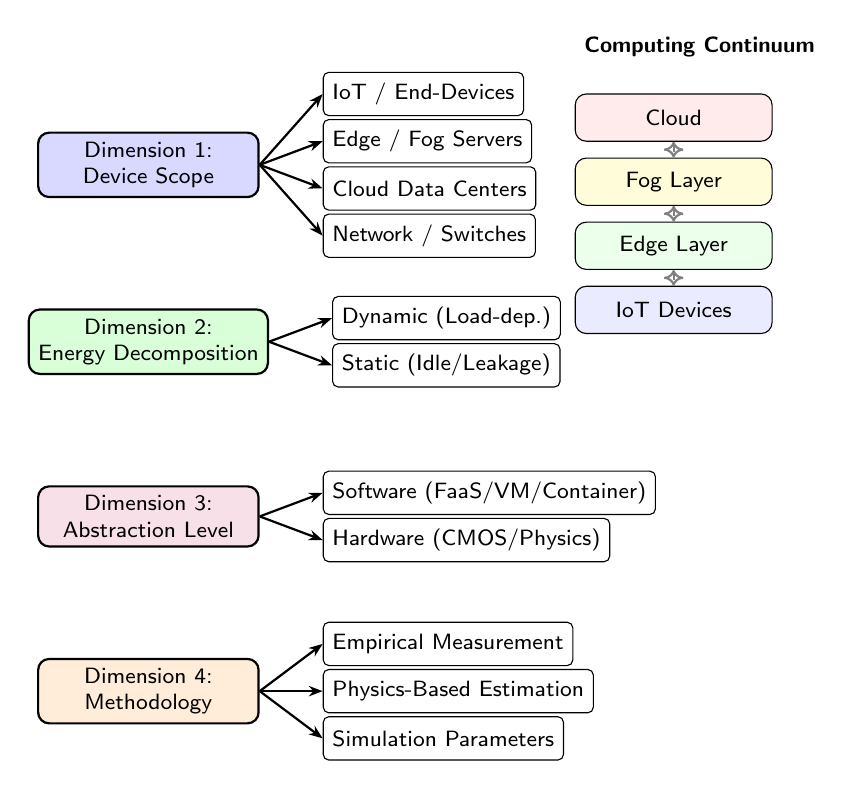
\begin{tikzpicture}[
    node distance=0.6cm and 1.2cm,
    every node/.style={font=\footnotesize},
    dimbox/.style={draw, rounded corners, minimum width=2.8cm, minimum height=0.7cm, align=center, thick},
    catbox/.style={draw, rounded corners=2pt, minimum width=2.2cm, minimum height=0.55cm, align=center, fill=white},
    arrstyle/.style={-{Stealth[length=5pt]}, thick},
    titlebox/.style={font=\footnotesize\bfseries, align=center}
]
% Dimension 1: Device Scope
\node[dimbox, fill=blue!15] (d1) {Dimension 1:\\Device Scope};
\node[catbox, right=0.8cm of d1, yshift=0.9cm] (iot) {IoT / End-Devices};
\node[catbox, right=0.8cm of d1, yshift=0.3cm] (edge) {Edge / Fog Servers};
\node[catbox, right=0.8cm of d1, yshift=-0.3cm] (cloud) {Cloud Data Centers};
\node[catbox, right=0.8cm of d1, yshift=-0.9cm] (net) {Network / Switches};
\draw[arrstyle] (d1.east) -- (iot.west);
\draw[arrstyle] (d1.east) -- (edge.west);
\draw[arrstyle] (d1.east) -- (cloud.west);
\draw[arrstyle] (d1.east) -- (net.west);

% Dimension 2: Energy Decomposition
\node[dimbox, fill=green!15, below=1.4cm of d1] (d2) {Dimension 2:\\Energy Decomposition};
\node[catbox, right=0.8cm of d2, yshift=0.3cm] (dyn) {Dynamic (Load-dep.)};
\node[catbox, right=0.8cm of d2, yshift=-0.3cm] (stat) {Static (Idle/Leakage)};
\draw[arrstyle] (d2.east) -- (dyn.west);
\draw[arrstyle] (d2.east) -- (stat.west);

% Dimension 3: Abstraction
\node[dimbox, fill=purple!12, below=1.4cm of d2] (d3) {Dimension 3:\\Abstraction Level};
\node[catbox, right=0.8cm of d3, yshift=0.3cm] (soft) {Software (FaaS/VM/Container)};
\node[catbox, right=0.8cm of d3, yshift=-0.3cm] (hard) {Hardware (CMOS/Physics)};
\draw[arrstyle] (d3.east) -- (soft.west);
\draw[arrstyle] (d3.east) -- (hard.west);

% Dimension 4: Methodology
\node[dimbox, fill=orange!15, below=1.4cm of d3] (d4) {Dimension 4:\\Methodology};
\node[catbox, right=0.8cm of d4, yshift=0.6cm] (meas) {Empirical Measurement};
\node[catbox, right=0.8cm of d4, yshift=0.0cm] (phys) {Physics-Based Estimation};
\node[catbox, right=0.8cm of d4, yshift=-0.6cm] (sim) {Simulation Parameters};
\draw[arrstyle] (d4.east) -- (meas.west);
\draw[arrstyle] (d4.east) -- (phys.west);
\draw[arrstyle] (d4.east) -- (sim.west);

% Continuum Architecture on the right
\node[titlebox, right=4.0cm of d1, yshift=1.5cm] (ctitle) {Computing Continuum};
\node[draw, rounded corners, fill=red!8, minimum width=2.5cm, minimum height=0.6cm, right=4.0cm of d1, yshift=0.6cm] (ccloud) {Cloud };
\node[draw, rounded corners, fill=yellow!15, minimum width=2.5cm, minimum height=0.6cm, below=0.2cm of ccloud] (cfog) {Fog Layer};
\node[draw, rounded corners, fill=green!8, minimum width=2.5cm, minimum height=0.6cm, below=0.2cm of cfog] (cedge) {Edge Layer};
\node[draw, rounded corners, fill=blue!8, minimum width=2.5cm, minimum height=0.6cm, below=0.2cm of cedge] (ciot) {IoT Devices};
\draw[<->, thick, dashed, gray] (ccloud.south) -- (cfog.north);
\draw[<->, thick, dashed, gray] (cfog.south) -- (cedge.north);
\draw[<->, thick, dashed, gray] (cedge.south) -- (ciot.north);
\end{tikzpicture}
}
\end{center}

\vspace{-0.3cm}

\textbf{Operational Energy Formulations:}
\vspace{-0.3cm}

\begin{itemize}
  \item \textbf{Server \& Cloud:} Modeled as a linear function of CPU utilization.
  \vspace{-0.1cm}

  \item \textbf{Holistic:} Sums computing hardware and cooling infrastructure overheads.
  \vspace{-0.1cm}

  \item \textbf{Analytical State-Based:} Integrates power over time for idle and active states.
  \vspace{-0.1cm}

  \item \textbf{Communication:} Link energy combines static switch and active per-port usage.
\end{itemize}

\textbf{Evaluation Methodologies:} 
\vspace{-0.3cm}
\begin{itemize}
  \item \textbf{Simulation Tools:} Scalable validation (e.g., CloudSim, iFogSim).
  \vspace{-0.1cm}
  \item \textbf{Experimental Testbeds:} Real-world setups for high-precision profiling.
\end{itemize}

}}
%----------------------------------------------------------------------------------------
%	Experimental Setup
%----------------------------------------------------------------------------------------
{\colorlet{headercol1}{benchmarkcol}\colorlet{headercol2}{benchmarkcol}
\headerbox{\textcolor{white}{Experimental Setup}}{name=experimental,span=3,column=3,row=1, below=introduction}{
\footnotesize


\vspace{0.1cm}
\begin{center}
  \textbf{Simulation Setup: Infrastructure and DSP}
\includegraphics[width=\linewidth]{SimulationSetup.png}
\end{center}

\vspace{0.15cm}
\begin{minipage}[c]{0.18\linewidth}
\centering
\includegraphics[width=\linewidth]{gcp.png}
\end{minipage}
\hfill
\begin{minipage}[c]{0.80\linewidth}
\begin{center}
\textbf{VMs GCE used in the case study (heterogeneous types)}

\vspace{0.2cm}
\begin{tabular}{l c c c c}
\toprule
\textbf{VM} & \textbf{Type GCP} & \textbf{vCPU} & \textbf{RAM (Go)} & \textbf{Zone} \\
\midrule
$v_1$ & e2-medium     & 2  & 4  & eu-west1-b \\
$v_2$ & e2-standard-4 & 4  & 16 & eu-west1-c \\
$v_3$ & n2-standard-2 & 2  & 8  & eu-west4-a \\
$v_4$ & e2-highcpu-4  & 4  & 4  & eu-east1-b \\
$v_5$ & n2-standard-4 & 4  & 16 & eu-west1-b \\
\bottomrule
\end{tabular}
\end{center}
\end{minipage}

\vspace{0.25cm}
\begin{minipage}[c]{0.18\linewidth}
\centering
\includegraphics[width=0.80\linewidth]{apache.png}
\end{minipage}
\hfill
\begin{minipage}[c]{0.85\linewidth}

\vspace{0.1cm}
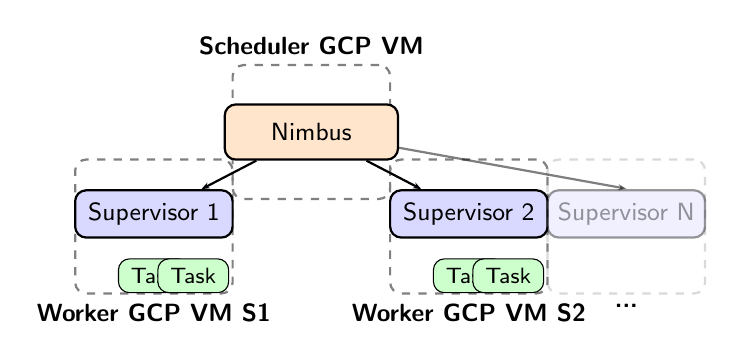
\begin{tikzpicture}[
node distance=1cm and 0.8cm,
every node/.style={font=\small},
scale=0.8,
nimbus/.style={draw, rounded corners, fill=orange!20, minimum width=2.2cm, minimum height=0.7cm, thick},
supervisor/.style={draw, rounded corners, fill=blue!15, minimum width=2cm, minimum height=0.6cm, thick},
task/.style={draw, rounded corners, fill=green!20, minimum width=0.9cm, minimum height=0.4cm, font=\footnotesize},
vm/.style={draw, dashed, rounded corners, minimum width=2cm, minimum height=1.7cm, thick, color=gray},
arrow/.style={-{Stealth[length=3pt]}, thick}
]

% VM1 - Supervisor 1
\node[vm, label={[font=\small]below:\textbf{Worker GCP VM S1}}] (vm1) at (0, 0) {};
\node[supervisor] (sup1) at (0, 0.2) {Supervisor 1};
\node[task, below=0.25cm of sup1] (task1) {Task};
\node[task, xshift=0.5cm, below=0.25cm of sup1] (task2) {Task};

% VM Nimbus - Centered above
\node[vm, label={[font=\small]above:\textbf{Scheduler GCP VM}}] (vmn) at (2.5, 1.5) {};
\node[nimbus] (nimbus) at (2.5, 1.5) {Nimbus};

% VM2 - Supervisor 2
\node[vm, label={[font=\small]below:\textbf{Worker GCP VM S2}}] (vm2) at (5, 0) {};
\node[supervisor] (sup2) at (5, 0.2) {Supervisor 2};
\node[task, below=0.25cm of sup2] (task3) {Task};
\node[task, xshift=0.5cm, below=0.25cm of sup2] (task4) {Task};

% VM3 - Partial box showing scalability
\node[vm, opacity=0.3, label={[font=\small]below:\textbf{...}}] (vm3) at (7.5, 0) {};
\node[supervisor, opacity=0.4] at (7.5, 0.2) {Supervisor N};

% Arrows from Nimbus to Supervisors
\draw[arrow] (nimbus) -- (sup1);
\draw[arrow] (nimbus) -- (sup2);
\draw[arrow, opacity=0.5] (nimbus) -- (7.5, 0.6);

\end{tikzpicture}
\begin{center}
\textbf{Storm Topology Deployment}
\end{center}

\end{minipage}
}
}

%----------------------------------------------------------------------------------------
%	Energy Results
%----------------------------------------------------------------------------------------
{\colorlet{headercol1}{benchmarkcol}\colorlet{headercol2}{benchmarkcol}
\headerbox{\textcolor{white}{Energy Simulation Results}}{name=results,span=3,column=3,row=1, below=experimental}{
\small
\begin{center}
\textbf{Energy Modeling and Algorithm Comparison}
\end{center}

\vspace{0.08cm}
{\footnotesize
We adopt a linear power model based on CPU utilization:
\begin{equation}\label{eq:power}
    P_j(u_j) = P_{idle,j} + (P_{max,j} - P_{idle,j}) \cdot u_j
\end{equation}


\vspace{0.08cm}
\begin{center}
\textbf{Placement Algorithm Comparison}
\vspace{0.08cm}

{\small
\begin{tabular}{l|c|c|c}
\toprule
\textbf{Metric} & \textbf{Greedy} & \textbf{CSP}\cite{ait2025optimisation} & \textbf{LLM (gemini-2.0)}\cite{ait2025optimisation} \\
\midrule
\textbf{$E_{total}$} (Wh) & 634785 & 265685 & 265685 \\
\textbf{Link Energy} (Wh) & 633500 & 265000 & 265000 \\
\textbf{Node Energy} (Wh) & 1285 & 685 & 685 \\
\textbf{$\mathcal{L}_{e2e}$} (ms) & 117 & 55 & 55 \\
\textbf{Solve Time} (s) & 0.000 & 5.314 & 1.076 \\
\textbf{Solver Cost} (Wh) & 0.000005 & 0.066422 & 0.000000 \\
\textbf{Active Hosts} & 6 & 3 & 3 \\
\bottomrule
\end{tabular}
}
\end{center}

\vspace{0.08cm}
{\footnotesize \textit{CSP and LLM achieve 58\% energy reduction compared to greedy FFD placement.}}
}
}}

%----------------------------------------------------------------------------------------
%	CONCLUSION
%----------------------------------------------------------------------------------------
\headerbox{Conclusion \& Perspectives}{name=conclusion,column=0,below=taxonomy,span=3}{
\textbf{Contributions:} Unified energy taxonomy and practical guidelines for task orchestration on GCP. \textbf{Mini-survey on energy aspects} across heterogeneous infrastructure. \textbf{Paper for COMPAS conference} documenting energy modeling and real-world benchmarking.

\textbf{Future Work:}
\vspace{-0.2cm}
\begin{itemize}
\item Scale experiments with larger and more heterogeneous VM infrastructures;
\vspace{-0.2cm}
\item Integrate link/network energy modeling into the optimization framework;
\vspace{-0.2cm}
\item Incorporate non-linear CPU power models for improved accuracy;
\vspace{-0.2cm}
\item Validate framework on real edge devices (Raspberry Pi clusters).
\end{itemize}
}

%----------------------------------------------------------------------------------------
%	REFERENCES
%----------------------------------------------------------------------------------------
\headerbox{References}{name=references,column=3,below=results, span=3}{
  \vspace{-0.5cm}
\smaller
\renewcommand{\refname}{}
\bibliographystyle{unsrt}
\bibliography{biblio}
}

\end{poster}

\end{document}